\documentclass[english, a4paper, oneside, onecolumn, openany,article]{memoir}
\usepackage{fix-cm,fixltx2e}
\usepackage{babel}  % babel: Hyphenation patterns and language specific strings
\usepackage{varioref}
\usepackage[colorlinks,linkcolor=black,urlcolor=black,citecolor=black]{hyperref}
\usepackage[colorinlistoftodos]{todonotes}
\usepackage[latin1]{inputenc}
\usepackage{graphicx}
\usepackage{listings}
\usepackage[square,numbers]{natbib}
\usepackage{url}
\usepackage{pslatex}
\usepackage{multirow}
\usepackage[T1]{fontenc}
\usepackage{eso-pic}
\usepackage{xcolor,calc}
\usepackage{pdfpages}
\newsubfloat{figure}
\usepackage{placeins} % gives me FloatBarrier
%Forhindrer floats i at flyde ind i næste afsnit
\let\oldsection=\section % gemmer den gamle definition
\renewcommand\section{\FloatBarrier\oldsection}

\makeatletter
\renewcommand\fps@figure{htbp} % Force figure placement
\renewcommand\fps@table{htbp}
\makeatother

% setup captions
\hangcaption
\changecaptionwidth
\captionwidth{9cm}


\title{Advanced Data Management - Assignment 1\\Value of Serializability}
\author{S\o ren Bjerregaard Vrist\\ITU Copenhagen}

\begin{document}
\maketitle

\chapter{Illustration of correctness}

\section{run.py}

\section{Results}
Based on the given \verb|run.py| I graphed two graphs. Figure
\ref{fig:origtime} and \ref{fig:origcorrect} is based on the output of
\verb|run.py|. We are trying to show that with ``restrictive'' isolation levels
- nearing on complete serialized with Repeatable read - you sacrifice
performance but gain correctness.
\begin{figure}
  \centering
  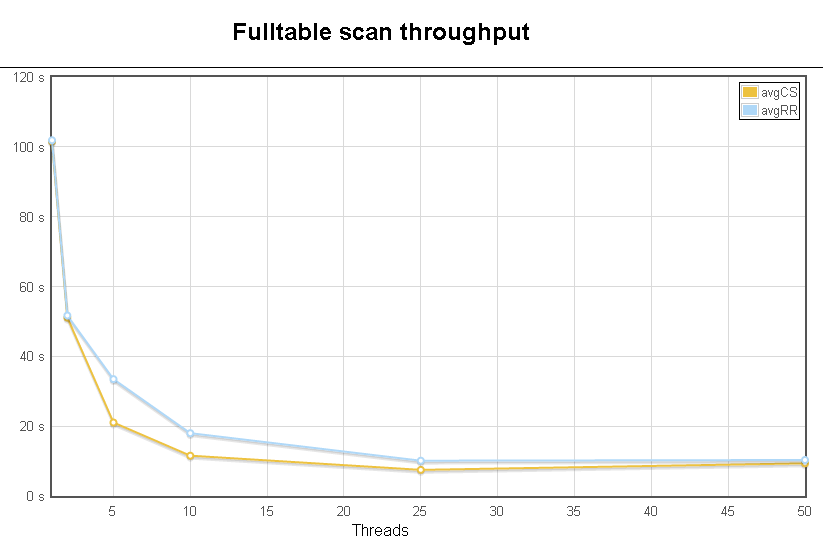
\includegraphics[width=10cm]{origtime}
  \caption[Average time over 5 runs]{Average time over 5 runs as a function of
  swap-threads for both Cursor Stability(CS) and Repeatable Read(RR) isolation levels.\\
  We would expect to non-neglible difference between CS and RR but to me it is
  not conclusive in this graph. The runtime is improved on increased parallelism
  for both isolation levels}\label{fig:origtime}
\end{figure}

Figure \ref{fig:origtime} shows the average runtime(y-axis) for 5 runs by run.py for
each level of concurrency (x-axis).


\begin{figure}
  \centering
  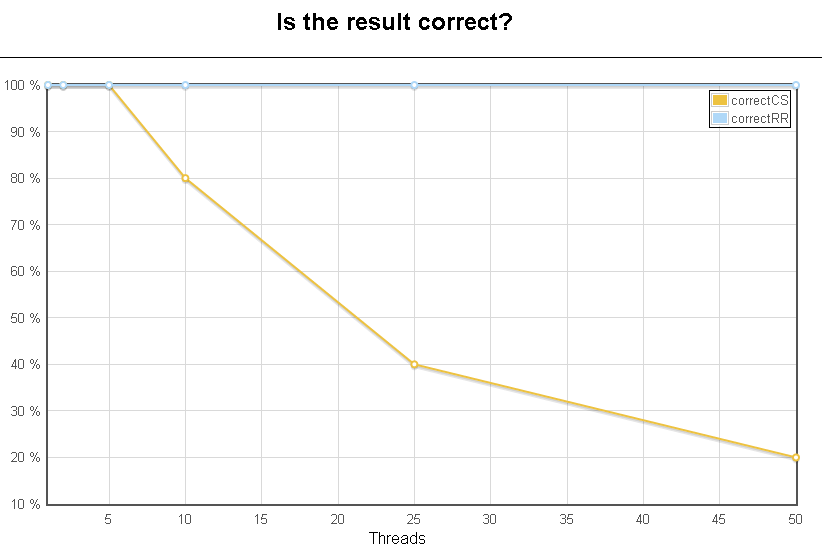
\includegraphics[width=10cm]{origcorrect}
  \caption{Average time over 5 runs as a function of swap-threads.}\label{fig:origcorrect}
\end{figure}

\section{Additional experiment}

%\begin{figure}
%\end{figure}


\section{Currently Committed}


\end{document}
